\section{Resolución mediante Backtracking}

Tal como concluimos en nuestro análisis teórico, al enfrentarnos a un problema NP-Completo como la selección de jugadores para contentar a la prensa (\textit{Hitting-Set}), sabemos que no existe un algoritmo de tiempo polinomial que nos garantice la respuesta óptima. Por lo tanto, para encontrar la lista mínima exacta de jugadores convocados, debemos recurrir a técnicas de búsqueda exhaustiva. 

Para este trabajo, implementamos un algoritmo de \textbf{Backtracking}. Esta técnica explora sistemáticamente todas las combinaciones posibles de jugadores (incluyéndolos o descartándolos de la lista final). Sin embargo, para evitar que el tiempo de ejecución se vuelva inmanejable incluso para listas pequeñas, le agregamos dos optimizaciones clave:
\begin{enumerate}
    \item \textbf{Pre-cálculo de coberturas:} Antes de empezar a explorar, armamos un diccionario que nos dice instantáneamente a qué medios de prensa contenta cada jugador.
    \item \textbf{Poda por optimalidad:} A medida que exploramos, guardamos el tamaño de la mejor lista de jugadores que encontramos hasta el momento. Si en una rama de la exploración vemos que la cantidad de jugadores seleccionados ya igualó o superó a nuestro récord actual, dejamos de explorar ese camino inmediatamente, ya que es matemáticamente imposible que mejore nuestra solución.
\end{enumerate}

A continuación, se presenta el código de nuestra solución en Python:

\begin{lstlisting}[language=Python, frame=single, numbers=left, breaklines=true, basicstyle=\ttfamily\footnotesize]
def hitting_set_backtracking(A, B):
    """
    A: Lista de elementos (jugadores disponibles).
    B: Lista de sets (cada set contiene los jugadores pedidos por un medio).
    """
    jugadores = list(A)
    n = len(jugadores)
    m = len(B)

    # Peor caso inicial: todos los jugadores
    mejor_solucion = list(A)

    # Para optimizar, precalculamos que conjuntos B_i cubre cada jugador
    # conjuntos_por_jugador[j] guardara los indices de los medios que lo quieren
    conjuntos_por_jugador = {j: set() for j in jugadores}
    for i, subset in enumerate(B):
        for jugador in subset:
            if jugador in conjuntos_por_jugador:
                conjuntos_por_jugador[jugador].add(i)

    def backtrack(idx, conjunto_actual, medios_cubiertos):
        nonlocal mejor_solucion

        # CASO BASE 1: Si se cubren a todos los medios de prensa
        if len(medios_cubiertos) == m:
            if len(conjunto_actual) < len(mejor_solucion):
                mejor_solucion = list(conjunto_actual)
            return

        # PODA: Si ya igualamos o superamos el tamano de la mejor solucion
        if len(conjunto_actual) >= len(mejor_solucion):
            return

        # CASO BASE 2: Si no hay mas jugadores pero no se cubrio a todos
        if idx == n:
            return

        jugador_actual = jugadores[idx]

        # OPCION 1: INCLUIR al jugador actual
        nuevos_medios = conjuntos_por_jugador[jugador_actual]
        medios_cubiertos_actualizado = medios_cubiertos | nuevos_medios

        conjunto_actual.append(jugador_actual)
        backtrack(idx + 1, conjunto_actual, medios_cubiertos_actualizado)
        conjunto_actual.pop()  # Deshacer cambio (Backtrack)

        # OPCION 2: NO INCLUIR al jugador actual
        backtrack(idx + 1, conjunto_actual, medios_cubiertos)

    # Llamada inicial
    backtrack(0, [], set())

    return mejor_solucion
\end{lstlisting}

\subsection*{Ejemplo de Ejecución}

Para corroborar la correctitud de la implementación, planteamos un pequeño set de datos simulando los deseos de cuatro medios de prensa sobre un plantel de seis jugadores:

\begin{lstlisting}[language=Python, frame=single, numbers=none, breaklines=true, basicstyle=\ttfamily\footnotesize]
jugadores_convocados = {"Messi", "Roncaglia", "Mateo Messi", "De Paul", "Dibujo Martinez", "Scaloni_Jr"}

prensa_deseos = [
    {"Roncaglia", "Messi"},        # Medio 1
    {"Mateo Messi"},               # Medio 2
    {"De Paul", "Mateo Messi"},    # Medio 3
    {"Dibujo Martinez", "Messi"}   # Medio 4
]
\end{lstlisting}

Al ejecutar nuestro algoritmo, el resultado obtenido es la lista \texttt{['Messi', 'Mateo Messi']}, cuyo tamaño es de 2 jugadores. Esto verifica empíricamente el funcionamiento del Backtracking: con solo citar a esos dos jugadores, Scaloni se asegura de que el Medio 1 y el Medio 4 estén contentos (por Messi), y que el Medio 2 y Medio 3 también lo estén (por Mateo Messi), logrando el subconjunto mínimo óptimo.

\subsection{Demostración empírica de tiempos y complejidad}

El algoritmo de resolución exacta diseñado mediante \textit{backtracking} se encuentra condicionado por dos variables principales: la cantidad de jugadores ($N$), que define el tamaño del universo, y la cantidad de conjuntos o medios a cubrir ($M$). Teóricamente, el algoritmo explora un árbol de decisión binario donde cada nodo representa la inclusión o exclusión de un jugador, lo que genera un espacio de estados en el peor de los casos de $O(2^N)$. Por otro lado, para cada configuración candidata, el algoritmo debe verificar de manera lineal la cobertura de las $M$ restricciones. En consecuencia, la complejidad teórica global responde al orden $O(M \cdot 2^N)$.

Para validar empíricamente este comportamiento, se generaron instancias sintéticas mediante el script \texttt{datos.py} y se registraron los tiempos de ejecución ejecutando \texttt{graficos.py}. A partir de los datos recolectados, se aplicó el método de mínimos cuadrados para evaluar y contrastar las hipótesis de complejidad.

\newpage
\subsubsection{Análisis variando la cantidad de jugadores ($N$)}

En primera instancia, se mantuvo fija la cantidad de conjuntos ($M=15$) y se barrió de forma creciente la cantidad de jugadores $N$. Como se observa en la Figura~\ref{fig:tiempos_n}, al contrastar el ajuste exponencial $O(2^N)$ contra un modelo polinomial alternativo $O(N^2)$, la curva exponencial acompaña con precisión el disparo vertical del tiempo de ejecución provocado por la explosión combinatoria.

\begin{figure}[H]
    \centering
    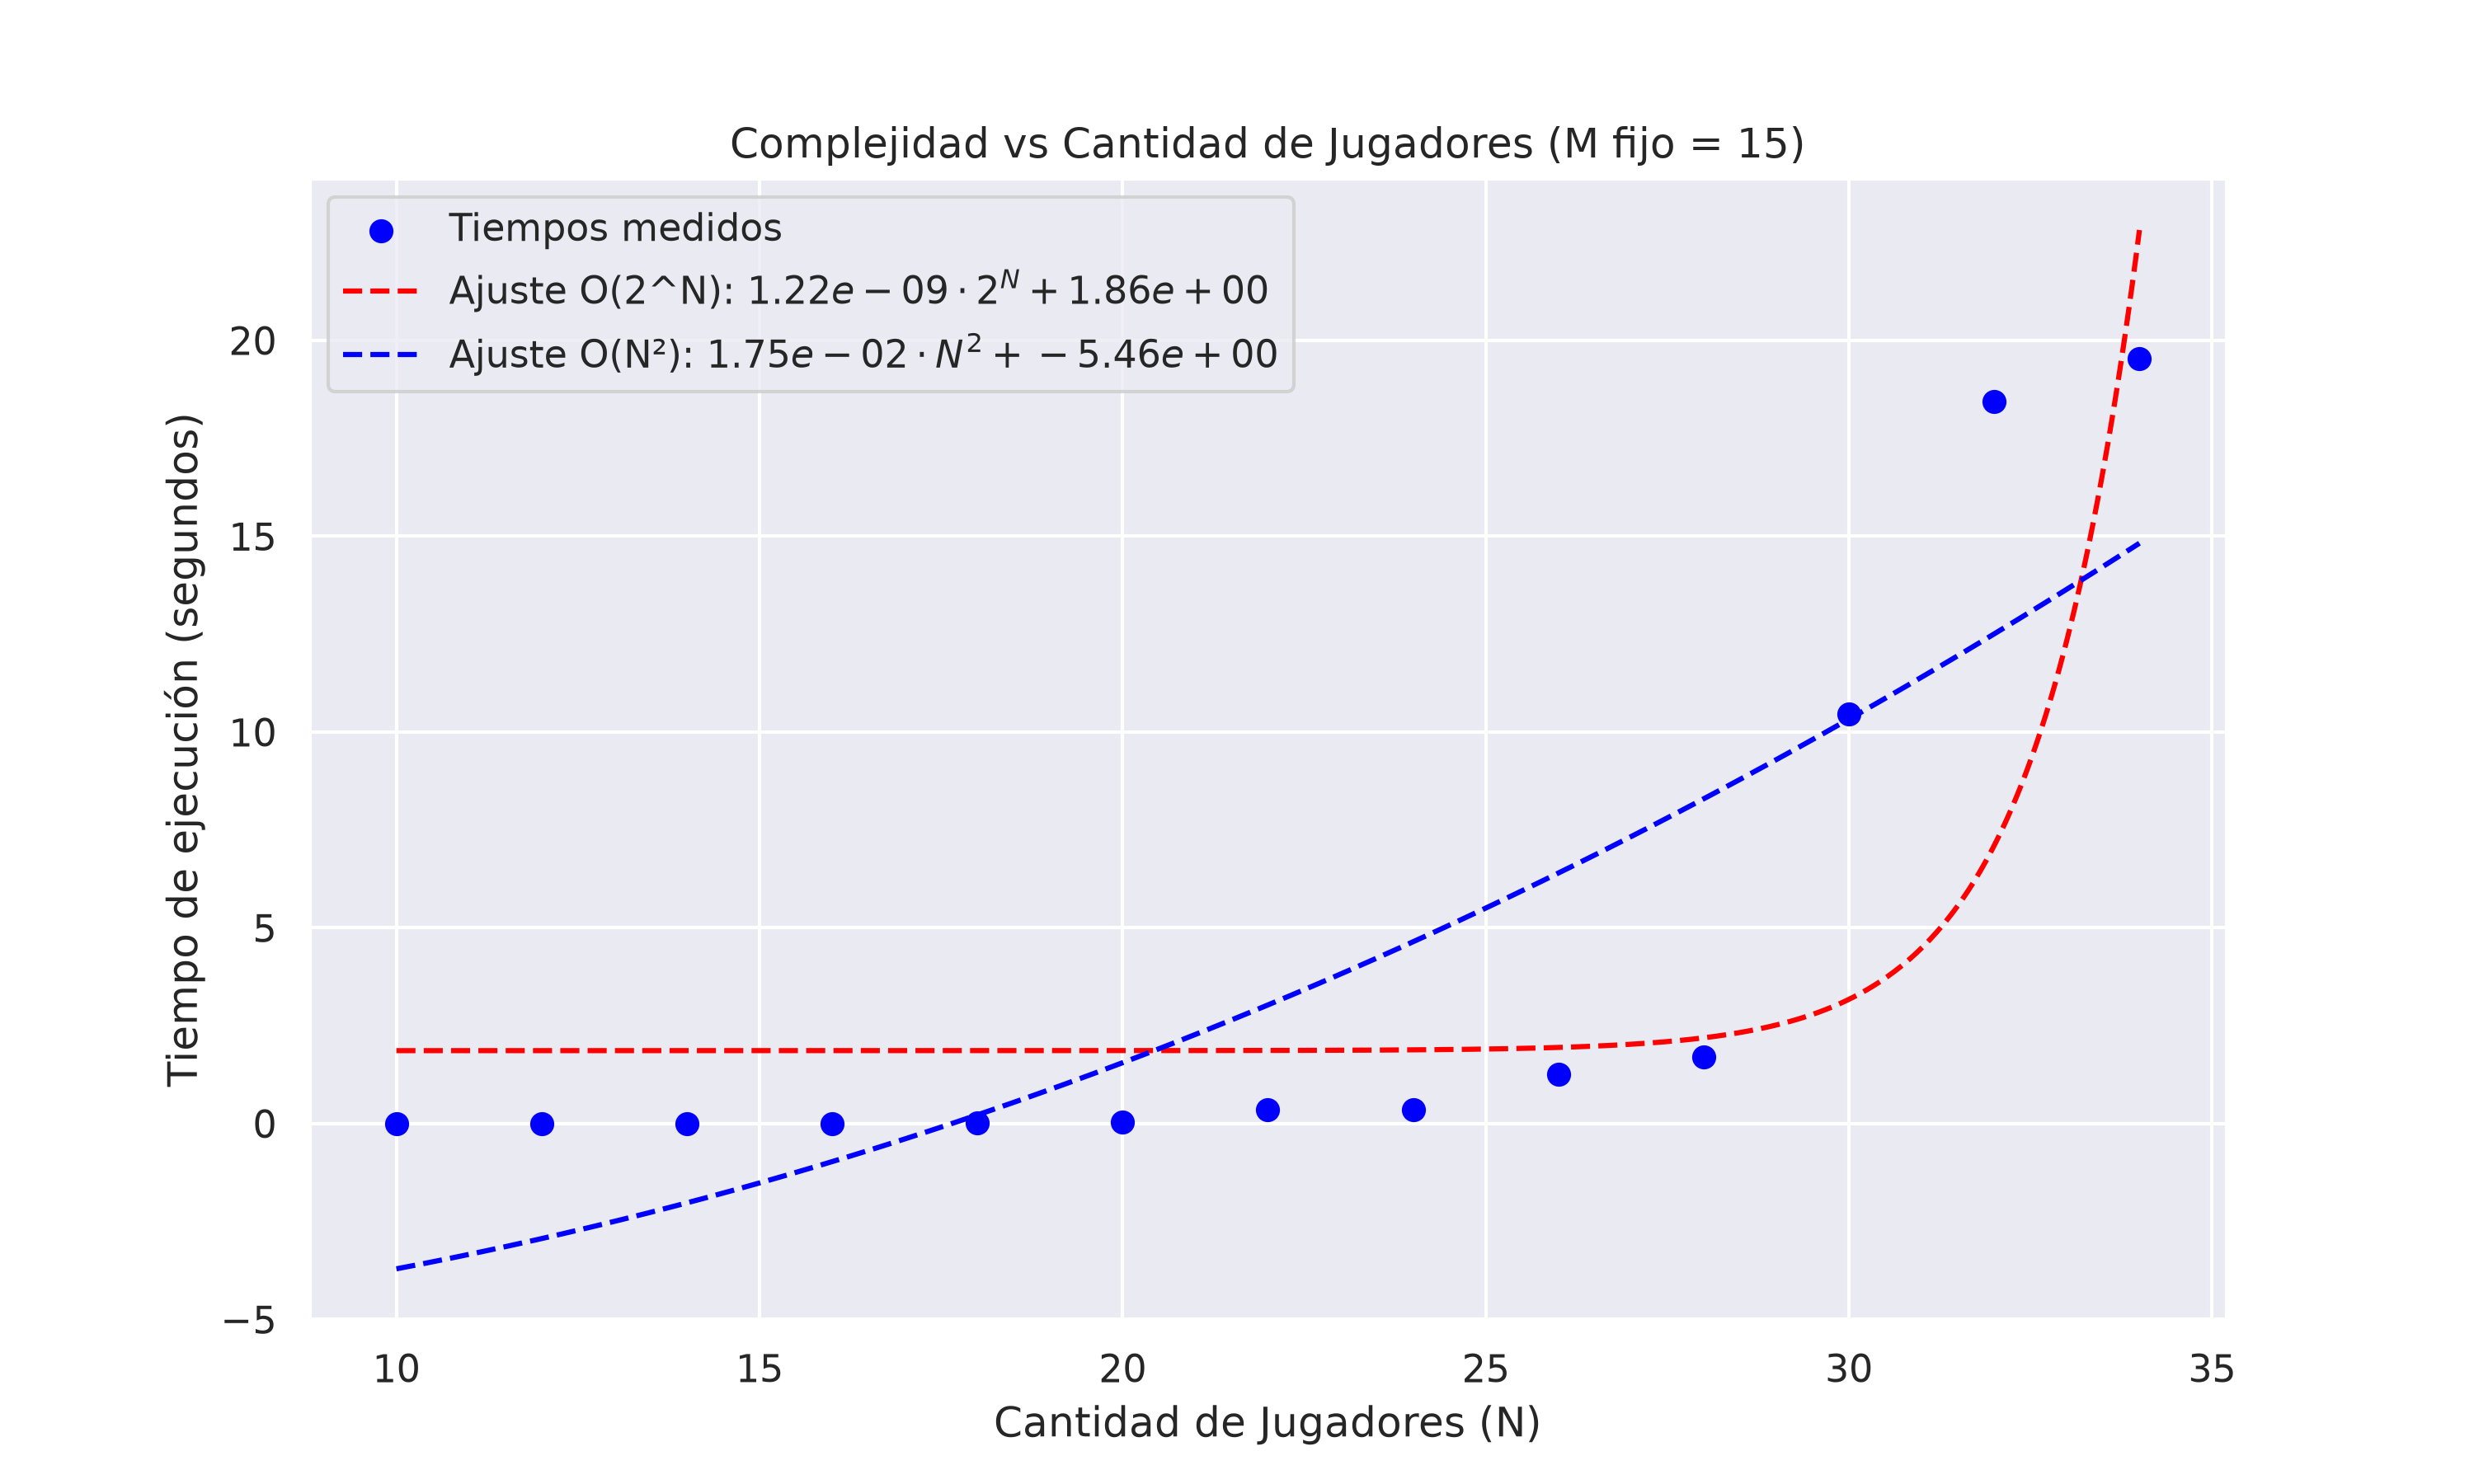
\includegraphics[width=0.85\textwidth]{img/tiempos_vary_n.png}
    \caption{Tiempo de ejecución en función de la cantidad de jugadores ($N$).}
    \label{fig:tiempos_n}
\end{figure}

Esta observación se convalida formalmente en la Figura~\ref{fig:error_n}, donde el gráfico de residuos muestra que el error absoluto del ajuste exponencial se mantiene drásticamente por debajo del error del modelo cuadrático, el cual es incapaz de modelar la aceleración asintótica del algoritmo.

\begin{figure}[H]
    \centering
    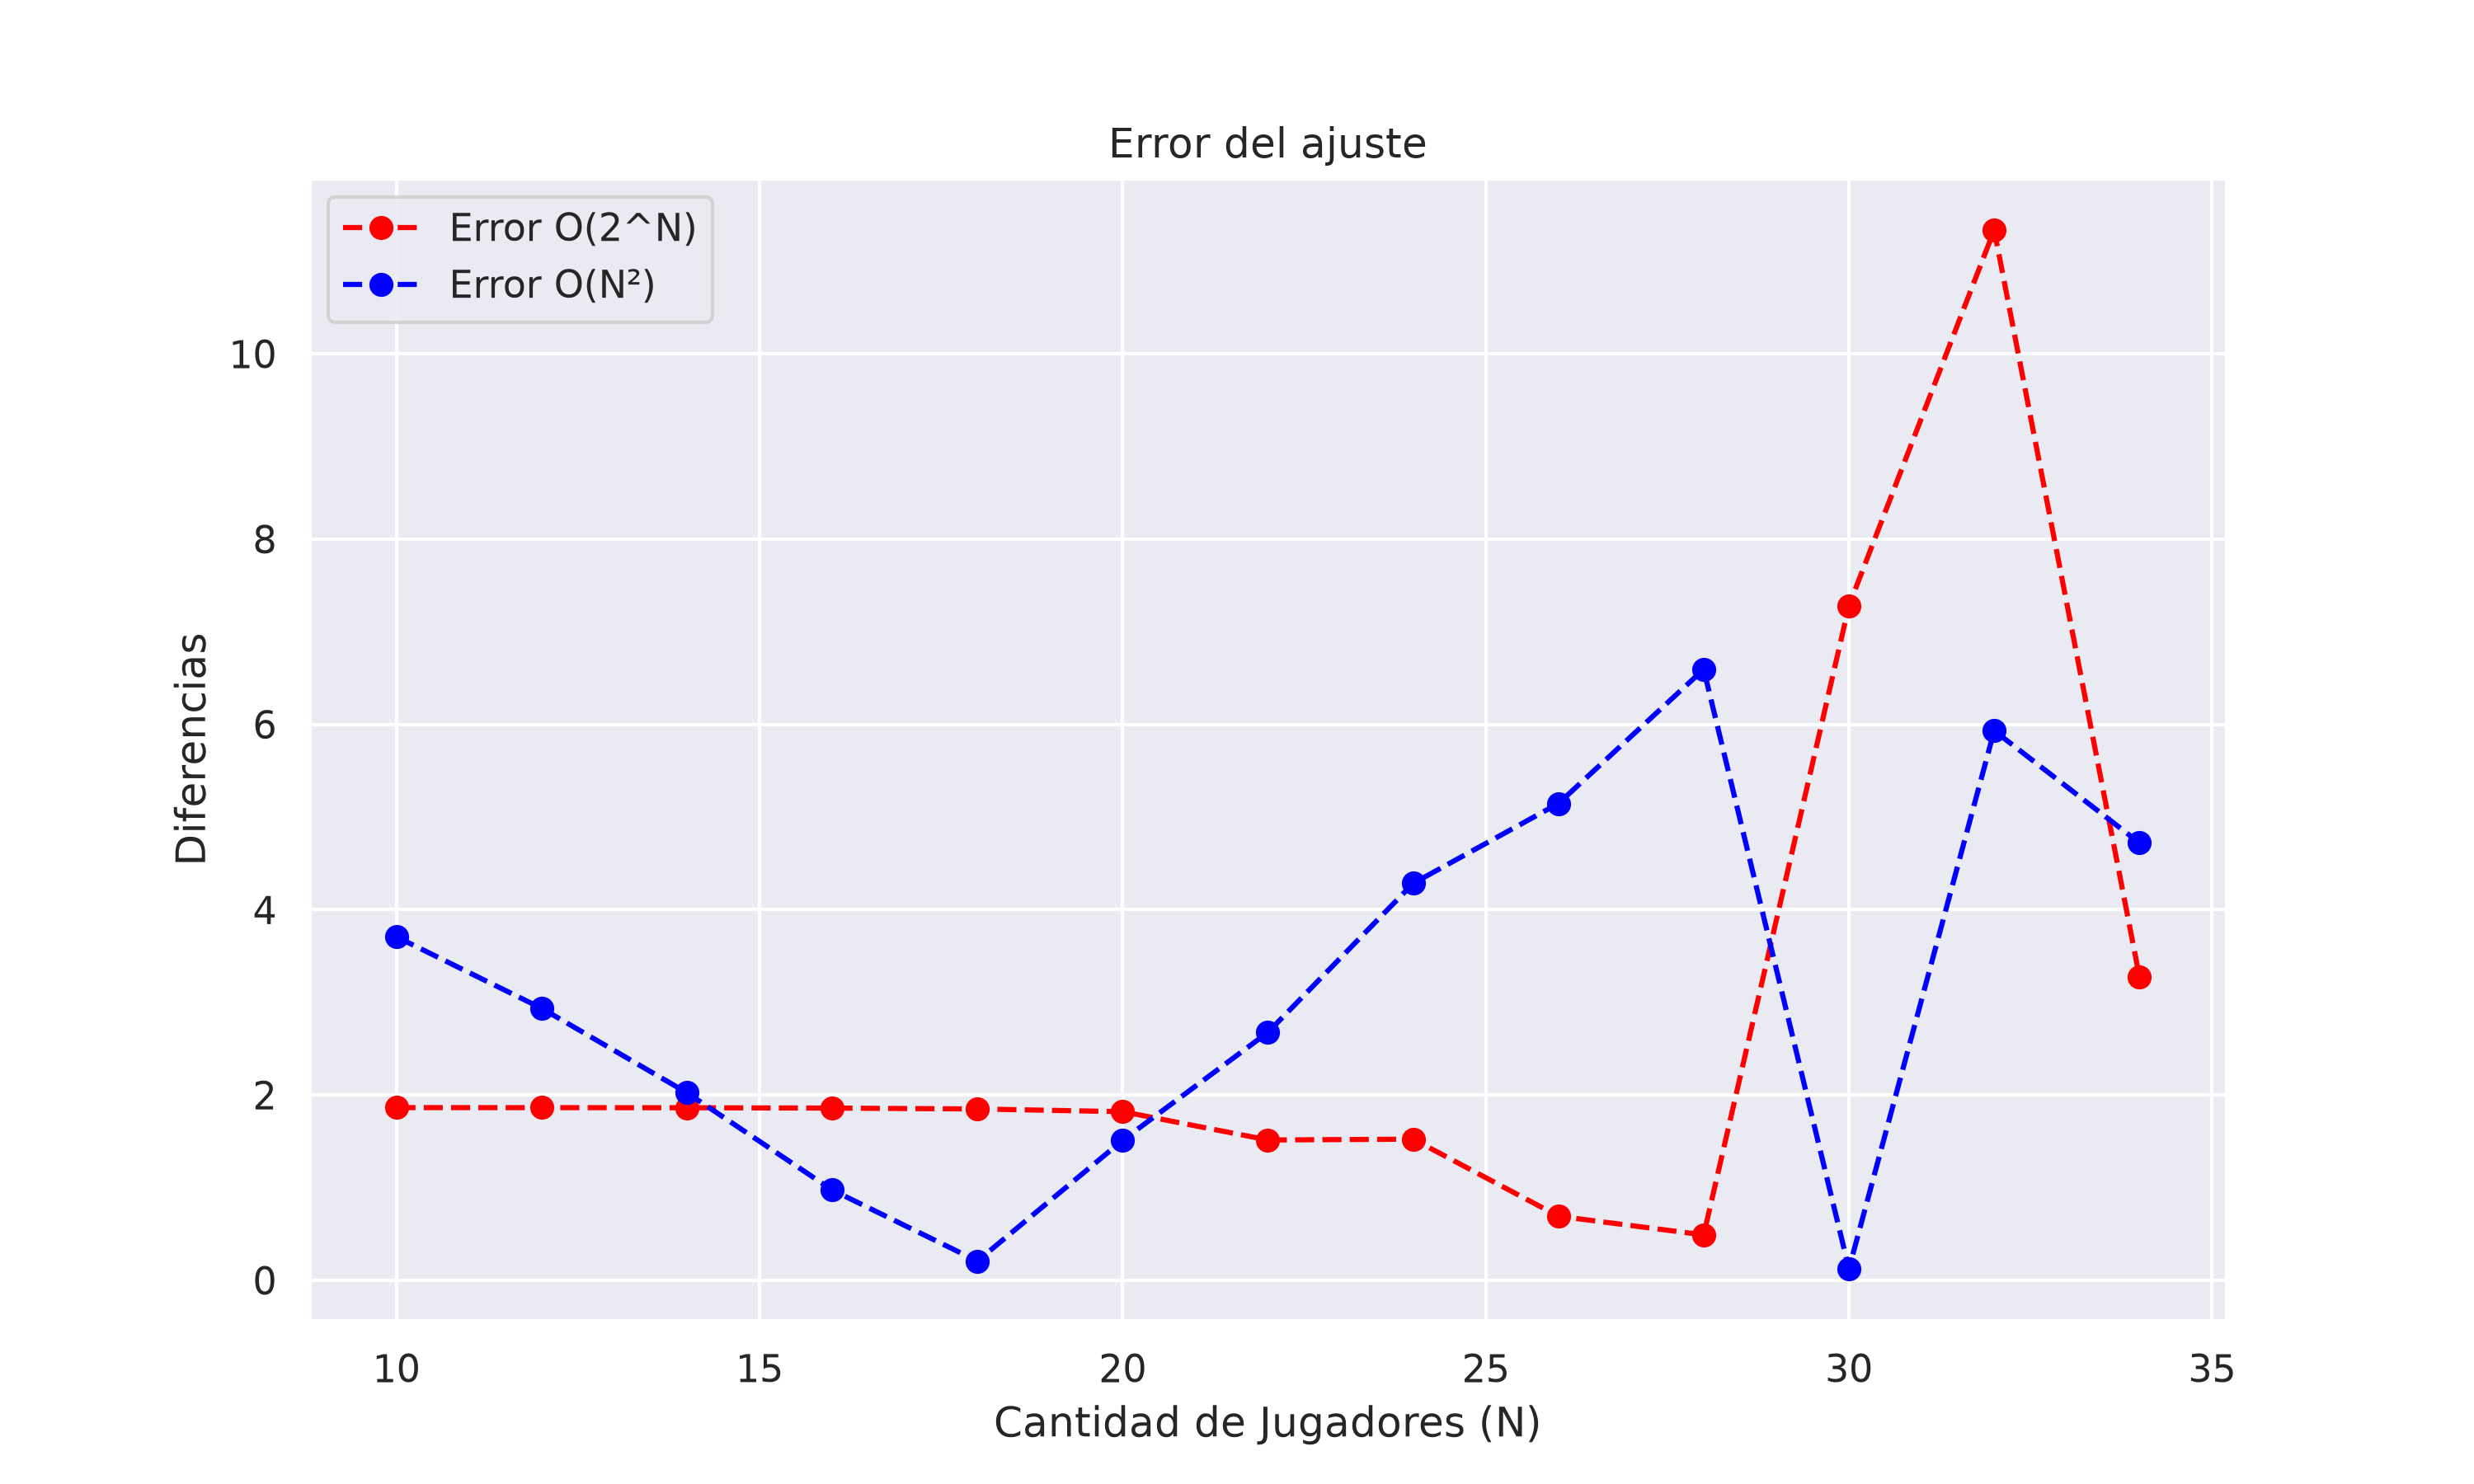
\includegraphics[width=0.85\textwidth]{img/error_vary_n.png}
    \caption{Error absoluto del ajuste para las hipótesis $O(2^N)$ y $O(N^2)$.}
    \label{fig:error_n}
\end{figure}

\subsubsection{Análisis variando la cantidad de conjuntos ($M$)}

Para estudiar el impacto de la cantidad de restricciones, se procedió a fijar la cantidad de jugadores en un valor constante ($N=25$) variando el parámetro $M$. Dado que el tamaño del árbol de backtracking permanece fijo, el tiempo de procesamiento pasa a depender exclusivamente de las verificaciones de cobertura sobre los conjuntos.

Al contrario de la experiencia anterior, el comportamiento esperado aquí es estrictamente \textbf{lineal}, es decir, $O(M)$. En la Figura~\ref{fig:tiempos_m} se evidencia que la nube de puntos describe una trayectoria rectilínea. Al contrastar el ajuste lineal $O(M)$ contra una hipótesis cuadrática $O(M^2)$, se aprecia que la recta se superpone perfectamente sobre los datos experimentales.

\begin{figure}[H]
    \centering
    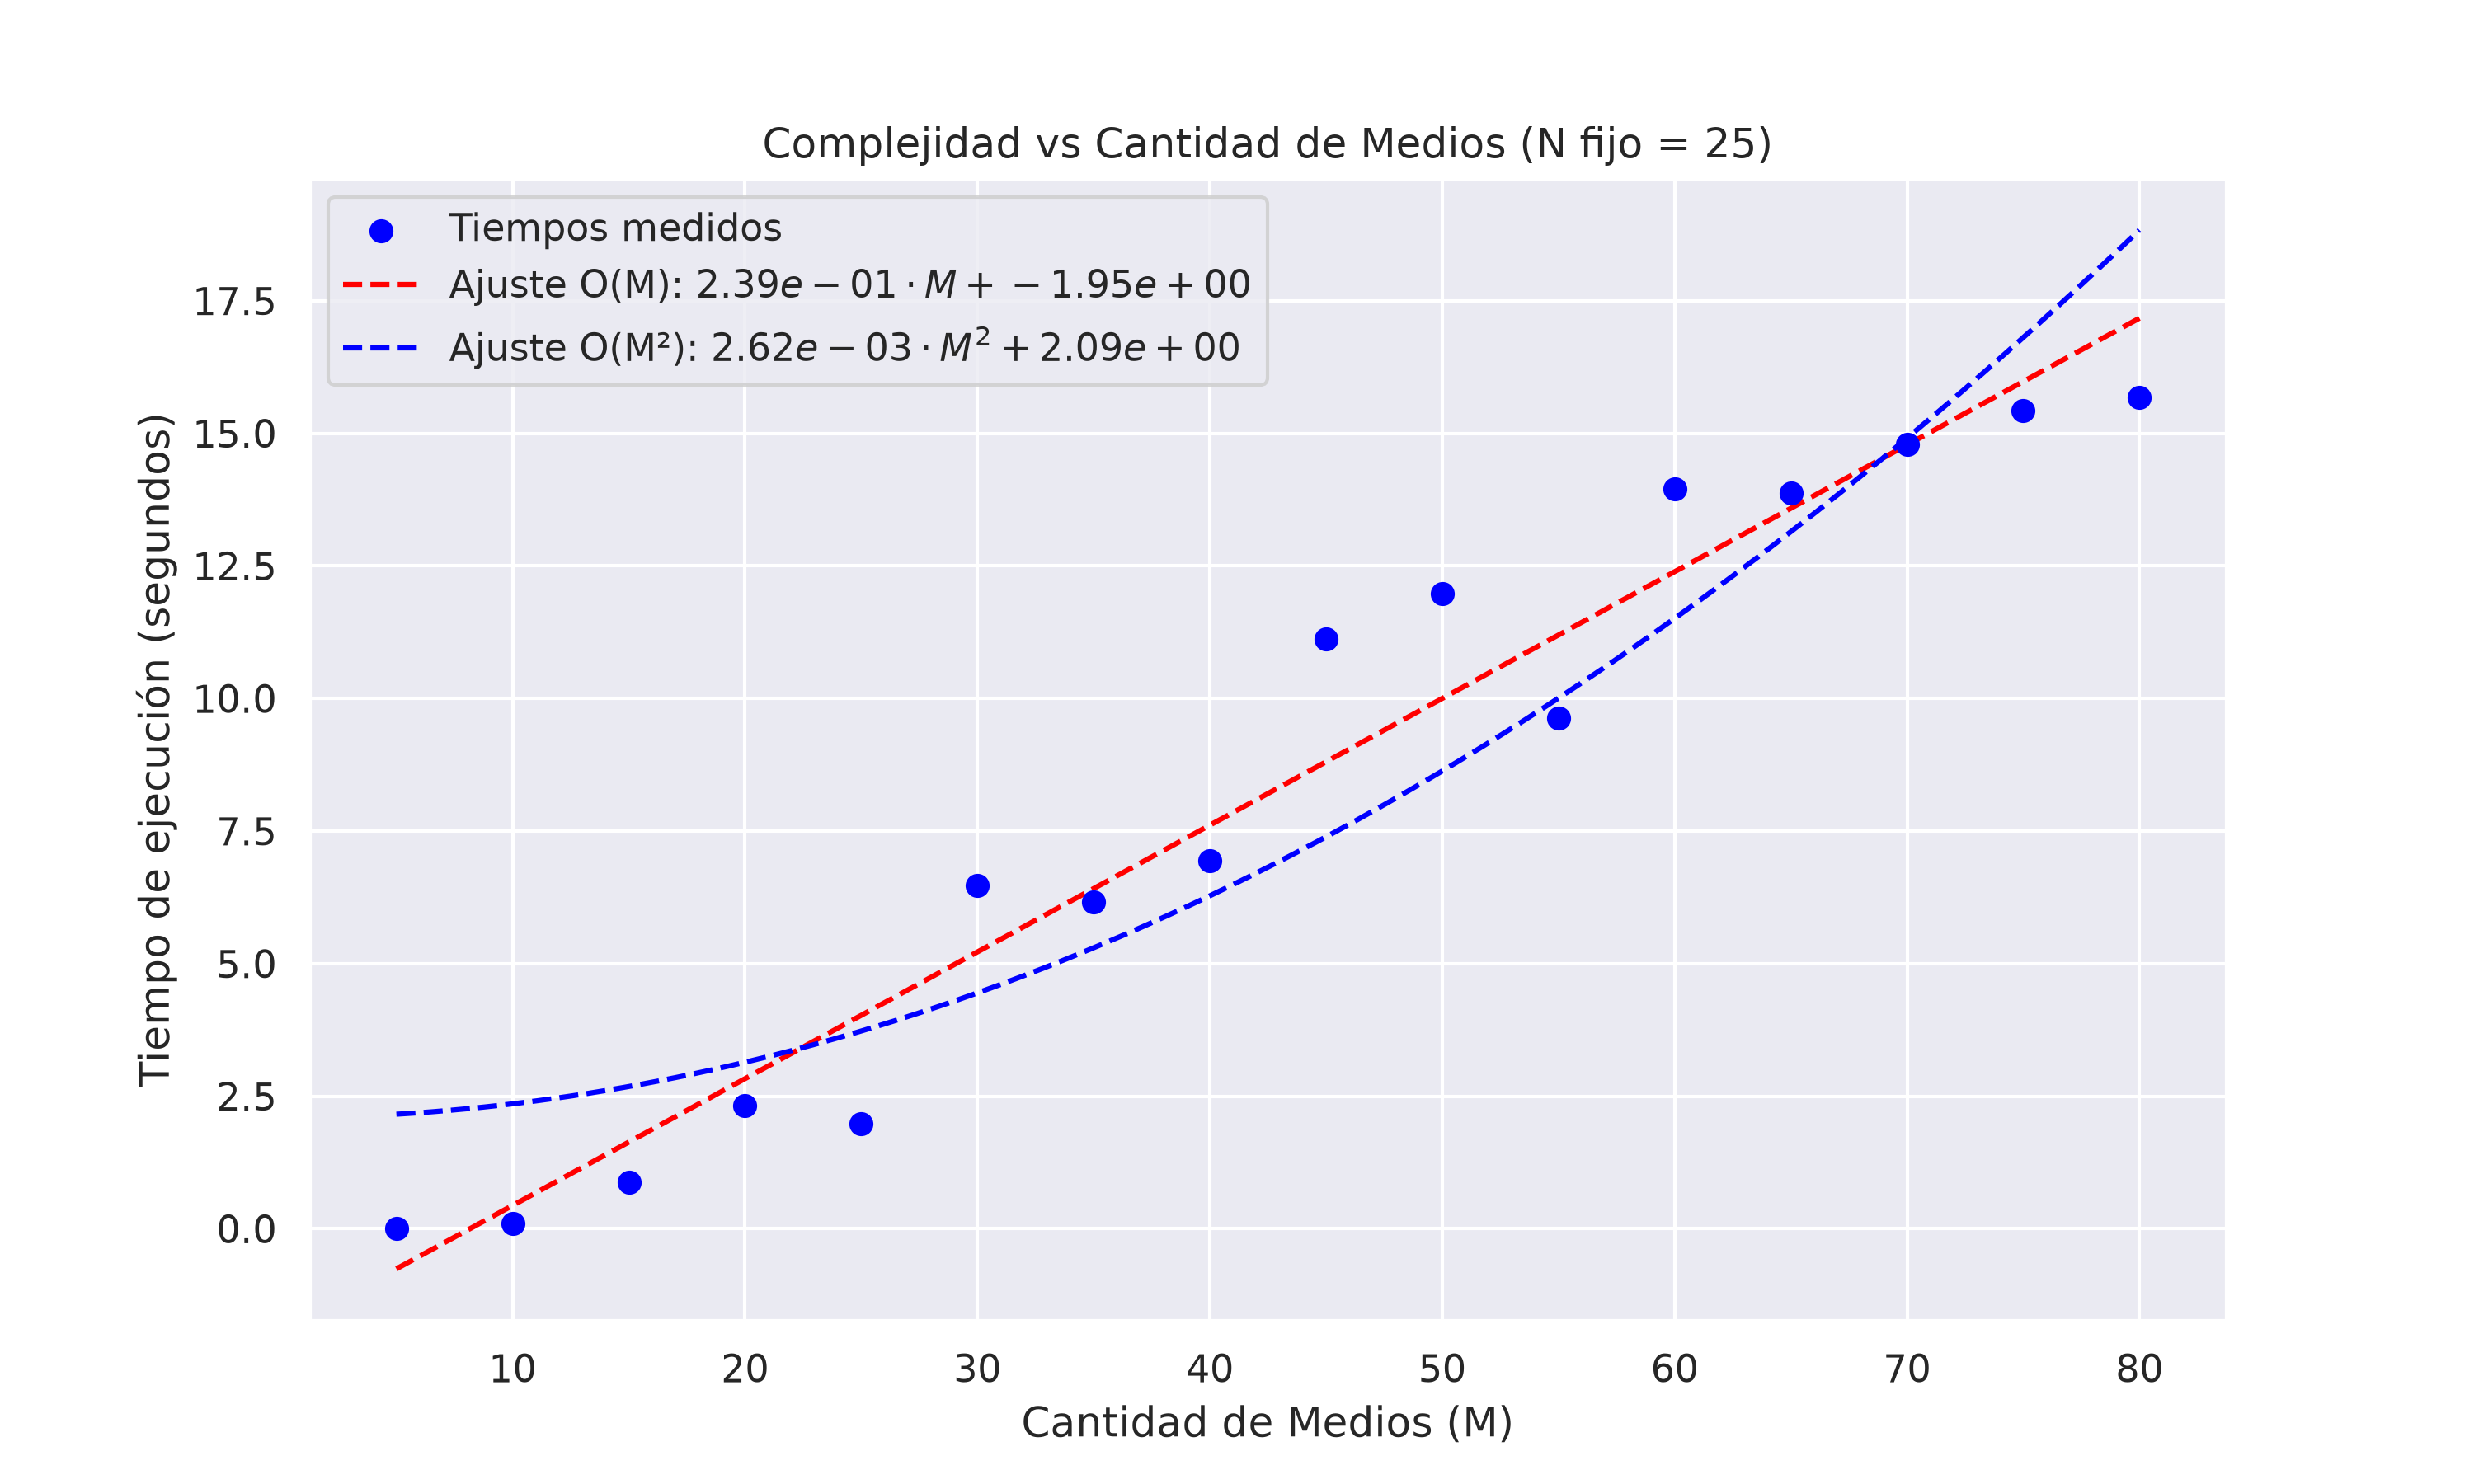
\includegraphics[width=0.85\textwidth]{img/tiempos_vary_m.png}
    \caption{Tiempo de ejecución en función de la cantidad de conjuntos ($M$).}
    \label{fig:tiempos_m}
\end{figure}

El análisis de residuos presentado en la Figura~\ref{fig:error_m} confirma esta conclusión: mientras que el error del modelo lineal fluctúa de forma acotada y muy cercana a cero, el error del modelo cuadrático se incrementa sistemáticamente en los extremos del dominio debido a que la parábola penaliza el ajuste intentando forzar una curvatura inexistente en la realidad empírica del programa.

\begin{figure}[H]
    \centering
    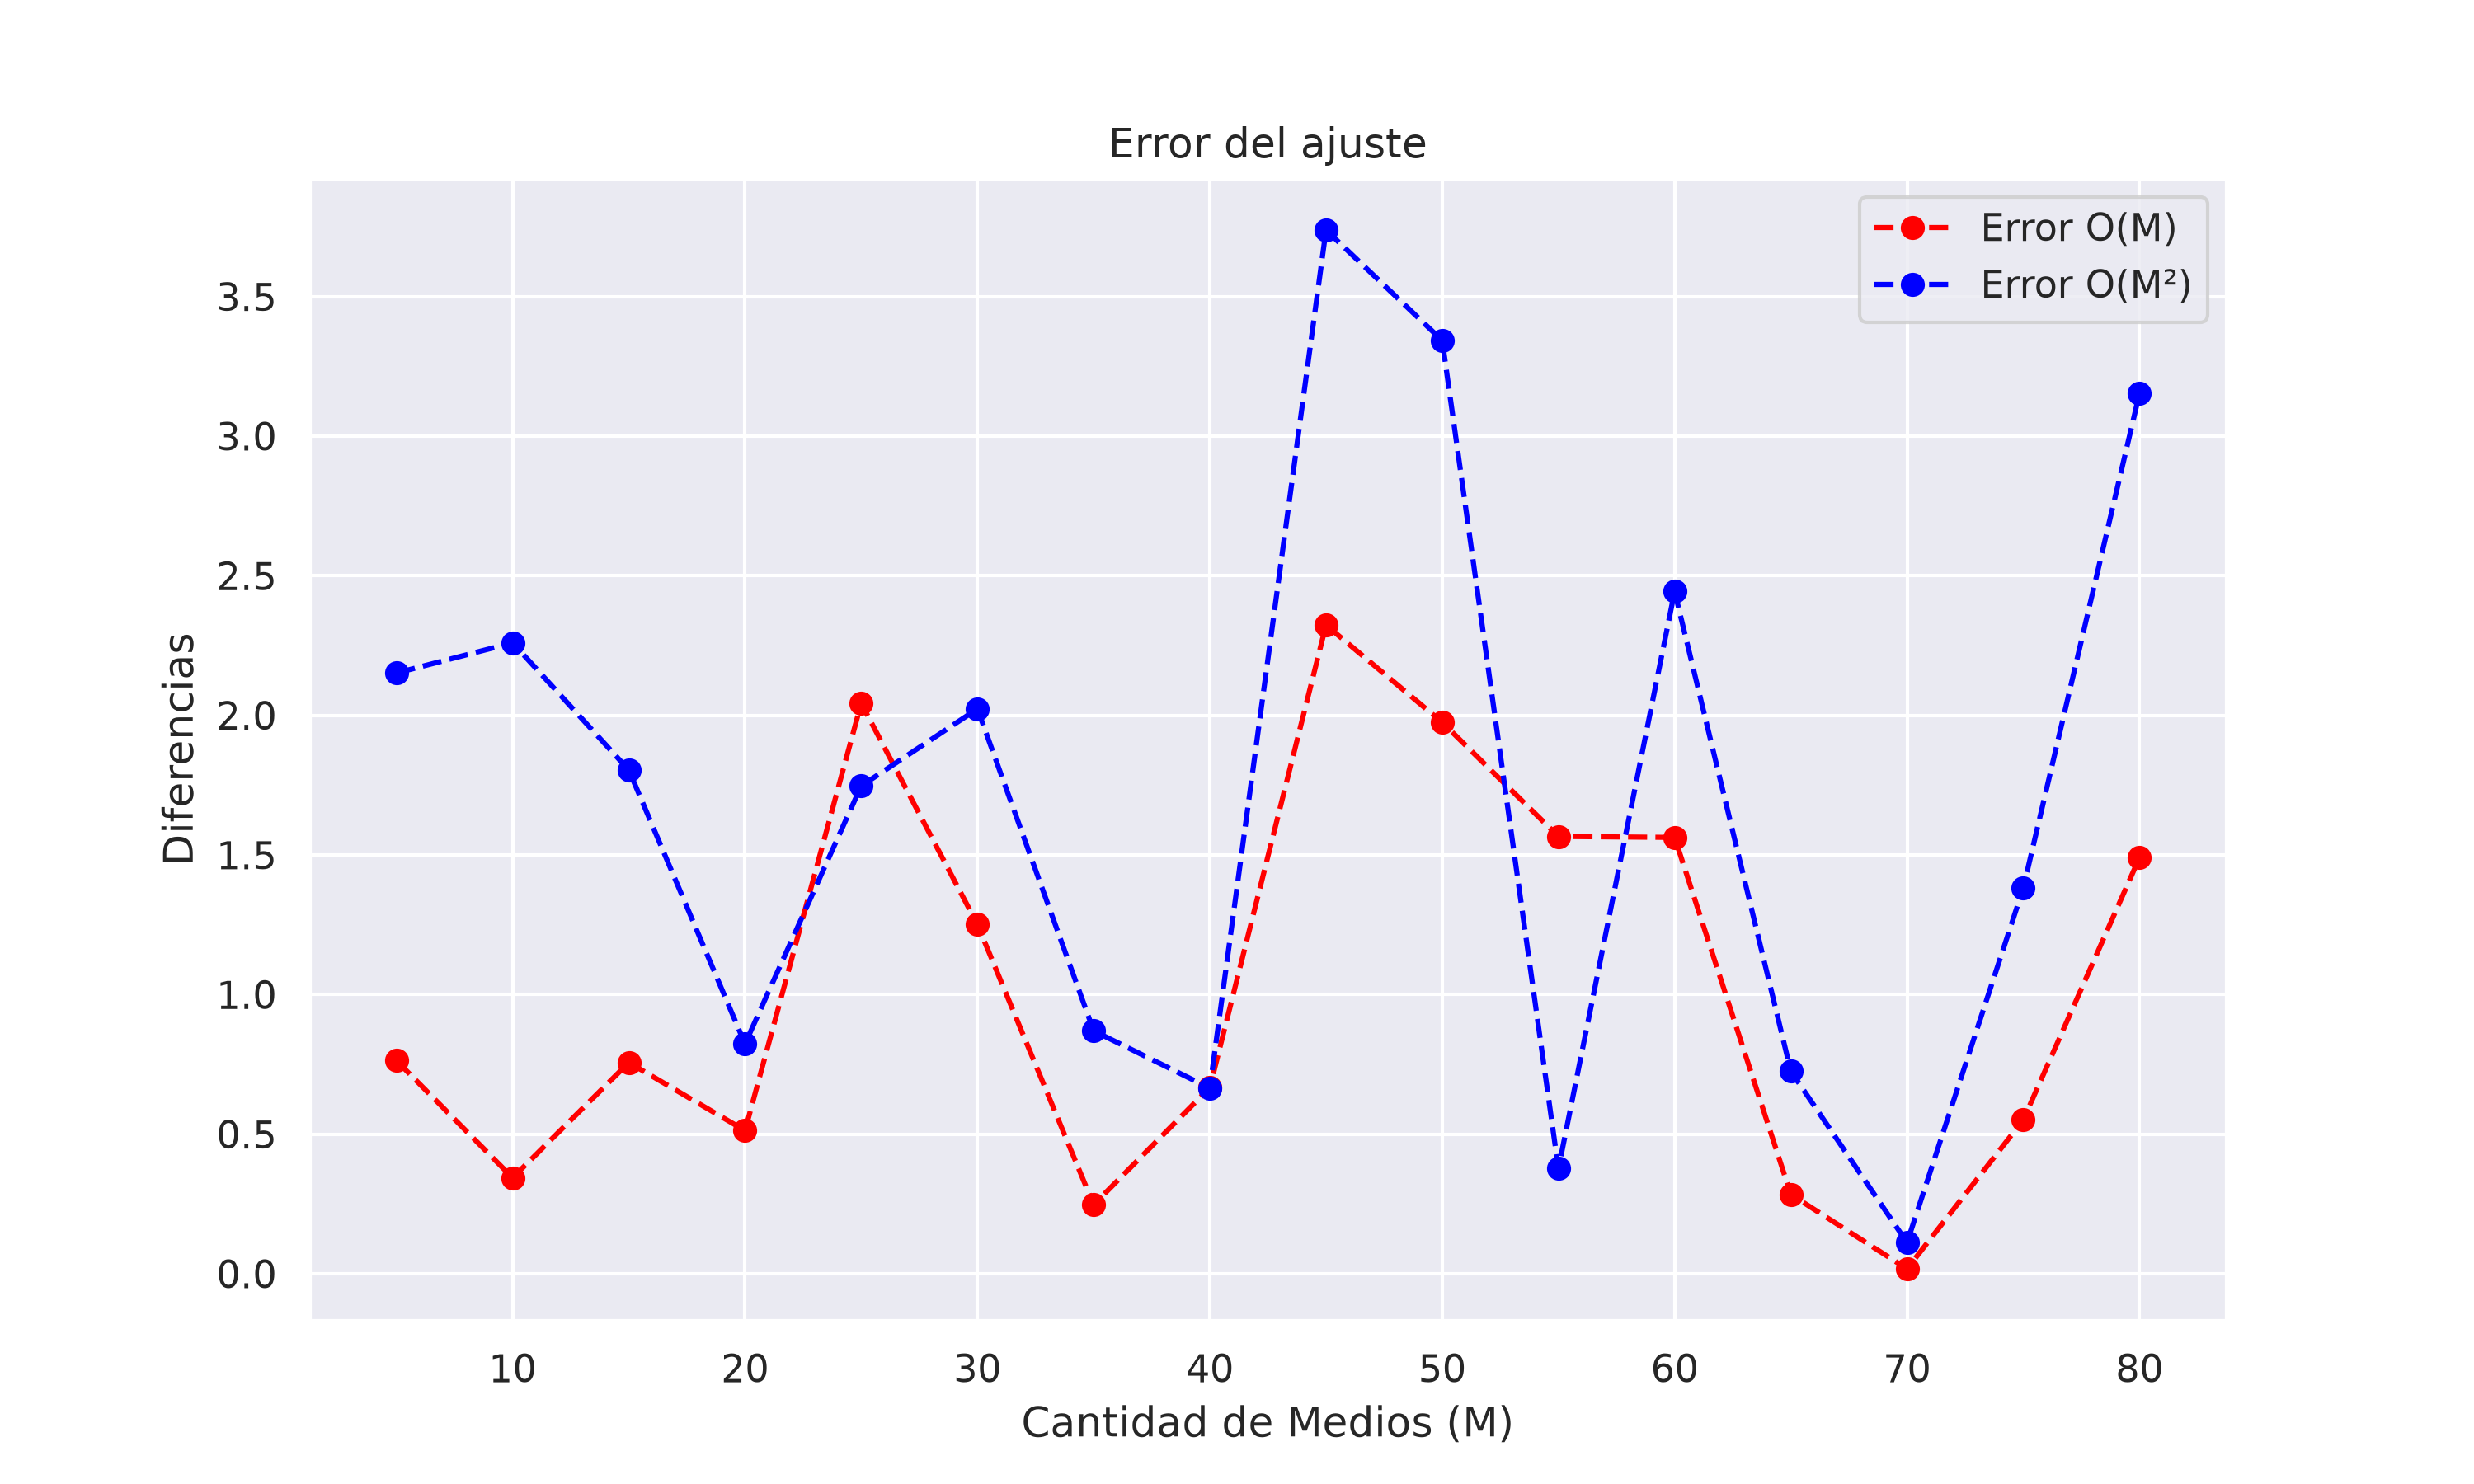
\includegraphics[width=0.85\textwidth]{img/error_vary_m.png}
    \caption{Error absoluto del ajuste para las hipótesis $O(M)$ y $O(M^2)$.}
    \label{fig:error_m}
\end{figure}